\documentclass[12pt]{article}
\usepackage{geometry}                % See geometry.pdf to learn the layout options. There are lots.
\geometry{letterpaper}                   % ... or a4paper or a5paper or ... 
%\geometry{landscape}                % Activate for for rotated page geometry
\usepackage[parfill]{parskip}    % Activate to begin paragraphs with an empty line rather than an indent
\usepackage{daves,fancyhdr,natbib,graphicx,dcolumn,amsmath,lastpage,url}
\usepackage{amsmath,amssymb,epstopdf,longtable}
\usepackage[final]{pdfpages}
\DeclareGraphicsRule{.tif}{png}{.png}{`convert #1 `dirname #1`/`basename #1 .tif`.png}
\pagestyle{fancy}
\lhead{CE 3354 -- Engineering Hydrology}
\rhead{FALL 2024}
\lfoot{ES3}
\cfoot{}
\rfoot{Page \thepage\ of \pageref{LastPage}}
\renewcommand\headrulewidth{0pt}



\begin{document}
\begin{center}
{\textbf{{ CE 3354 Engineering Hydrology} \\ {Exercise Set 3}}}
\end{center}

\section*{\small{Exercises}}
\begin{enumerate}
\item  Figure \ref{fig:RainfallData} is a portion of the spreadsheet named \texttt{RainfallData.xlsx} that contains cumulative rainfall for a gage in Dallas, Texas.   Convert/interpolate the data into 15-minute cumulative rainfall (amount of rainfall every 15 minutes).   Be aware the cumulative data is irregular in time (there are variable $\Delta t$ values in the data). \\

\begin{figure}[h!] %  figure placement: here, top, bottom, or page
   \centering
   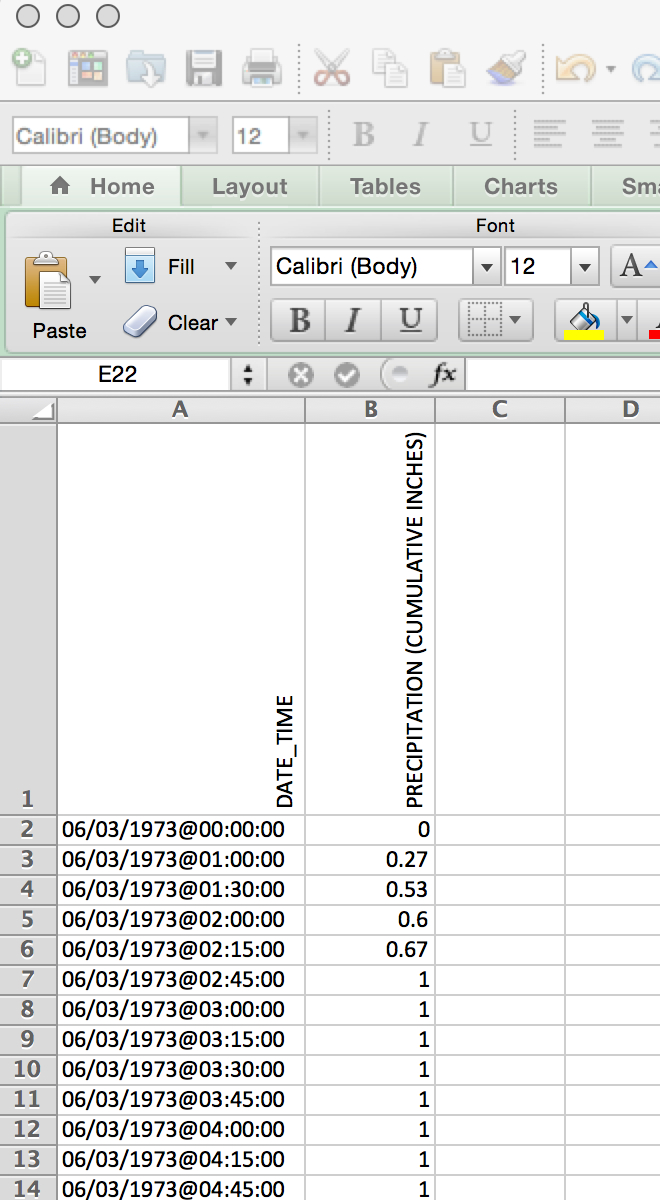
\includegraphics[height=4in]{RainfallData.jpg} 
   \caption{Portion of Rainfall Data spreadsheet.}
   \label{fig:RainfallData}
\end{figure}

\item Convert the 15-minute cumulative rainfall into 15-minute incremental rainfall. \\
\clearpage
\item  Figure \ref{fig:RunoffData} is a portion of the spreadsheet named \texttt{RunoffData.xlsx} that contains runoff for a gage in Dallas, Texas as specific moments in time.   Convert/interpolate the data into 15-minute cumulative runoff.   The drainage area is 6.92 miles.  Express the result in watershed inches of runoff.  Be aware the data is irregular in time (there are variable $\Delta t$ values in the data). \\

\begin{figure}[h!] %  figure placement: here, top, bottom, or page
   \centering
   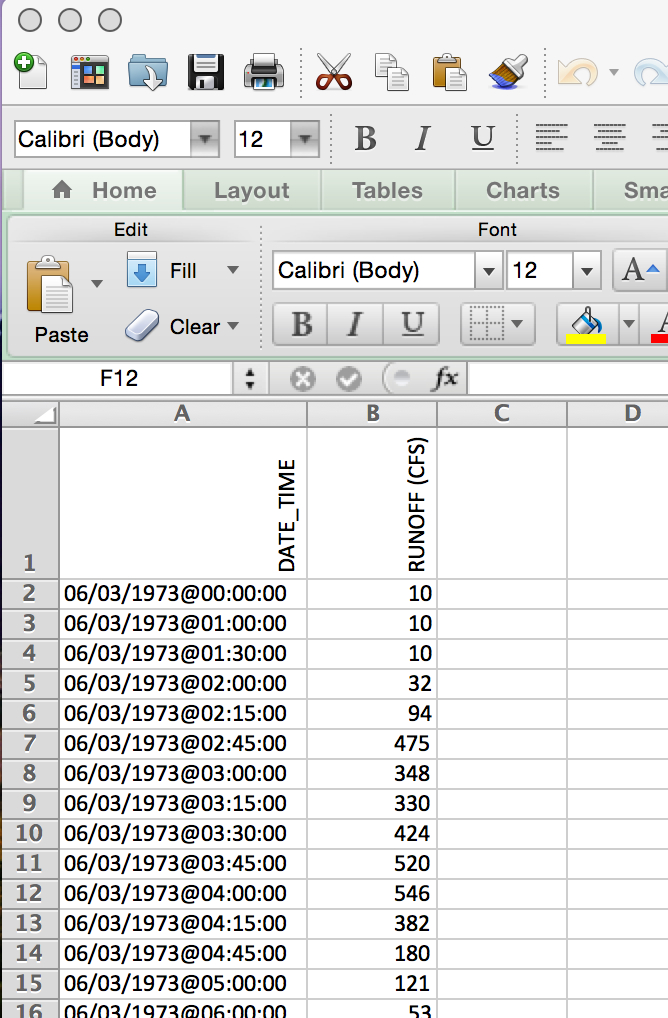
\includegraphics[height=4in]{RunoffData.jpg} 
   \caption{Portion of Runoff Data spreadsheet.}
   \label{fig:RunoffData}
\end{figure}

\item Plot the 15-minute cumulative rainfall and the 15-minute cumulative runoff (in watershed inches) on the same time axis.   What do these plots look like? \\

\clearpage
\item Figure \ref{fig:OklahomaData} The following data represent gage height and annual peak discharge for some gaging station in Oklahoma.  The stage is in feet and the discharge is in cubic feet per second.  The data are sequential from 1923 through 1971.

\begin{figure}[h!] %  figure placement: here, top, bottom, or page
   \centering
   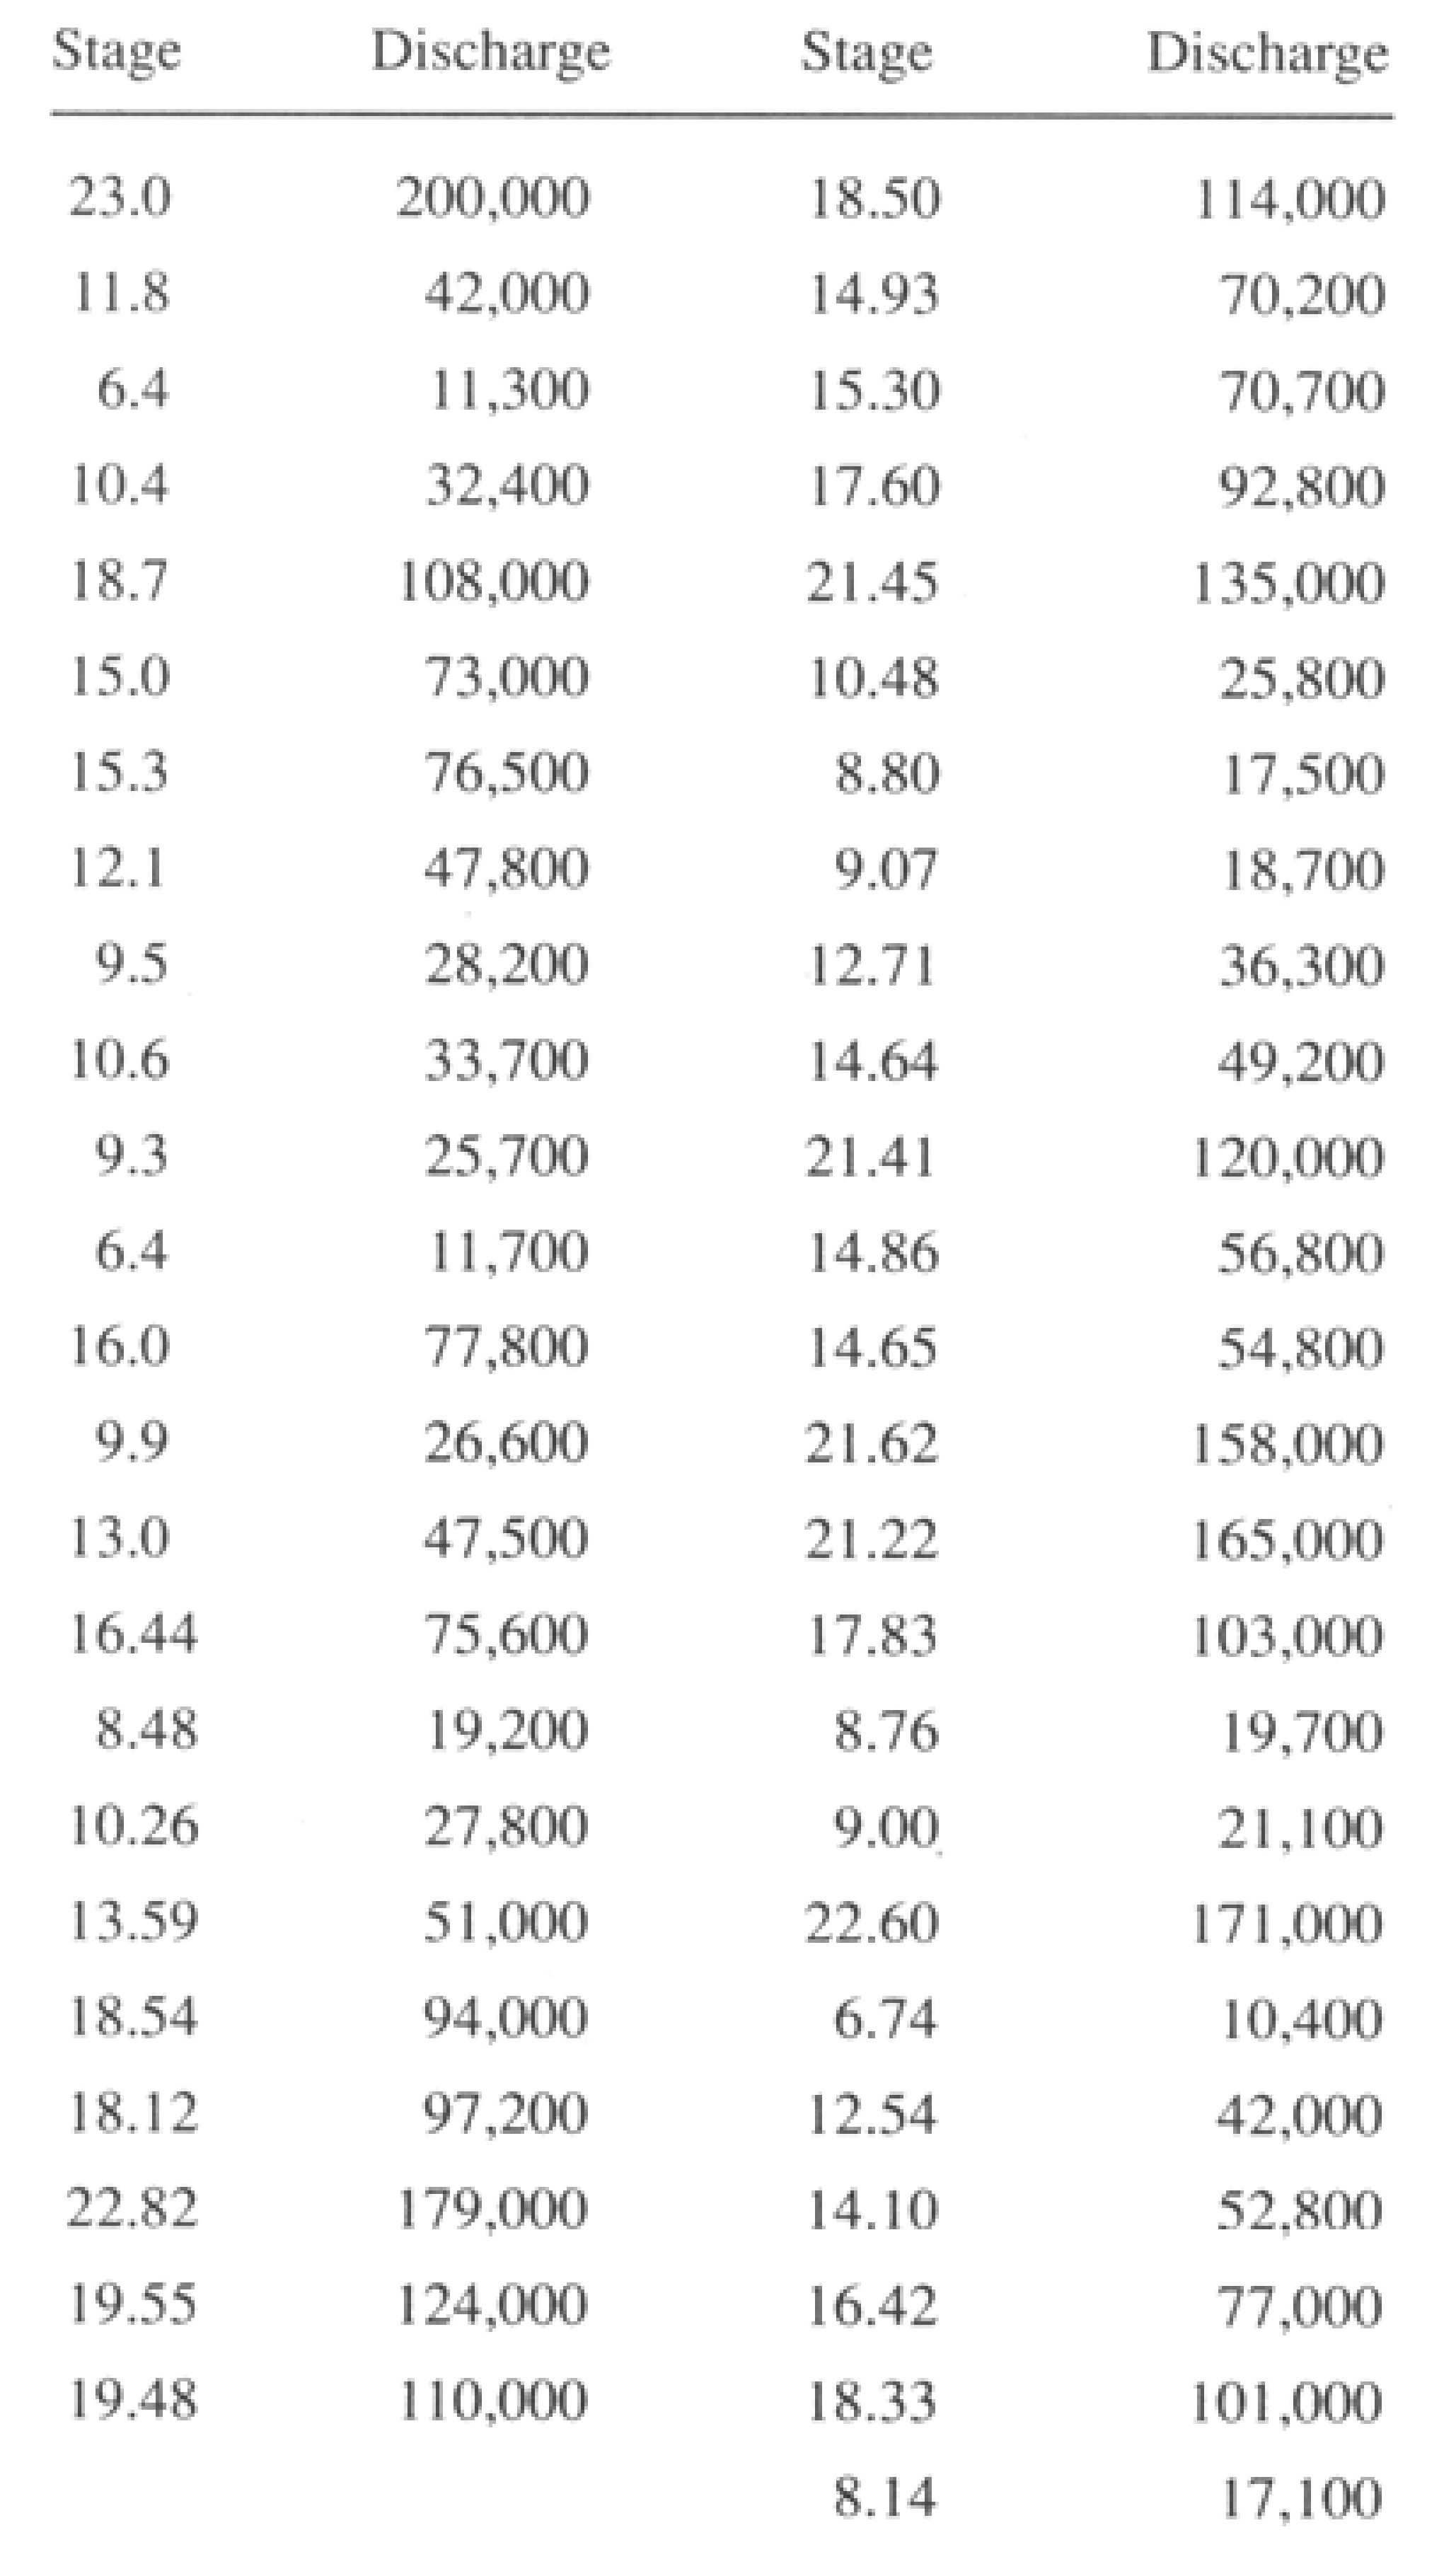
\includegraphics[height=7in]{OklahomaData.jpg} 
   \caption{Data from Oklahoma Gaging Station}
   \label{fig:OklahomaData}
\end{figure}


Use the data to:
\begin{enumerate}
\item Plot year versus stage ( x-axis is year).
\item Plot year versus discharge ( x-axis is year).
\item Plot the discharge versus stage.
\item Using the Weibull plotting position formula, determine the distribution parameters that fit the data for a log-normal distribution.
\item Using the Weibull plotting position formula, determine the distribution parameters that fit the data for a Gumbell distribution.
\item Using the Weibull plotting position formula, determine the distribution parameters that fit the data for a Gamma distribution.
\item Estimate the discharge associated with a 25-percent chance exceedence probability (i.e. the value that is equal to or exceeded with a 1 in 4 chance).
\item A resident claims that in the early 1900?s a flood corresponding to a stage of 30 feet occurred at the gage location.  Estimate the exceedence probability (return period) of the flow assicoated with this event.
\end{enumerate}

\textbf{Save these data, you will reuse them in Flood Frequency Analysis Bulletin 17C software later on.}

\end{enumerate}


\end{document}  